\chapter{Kyberhyökkäyksiltä suojautuminen}\label{suojautuminen}

Esittelen seuraavaksi keinoja suojautua aikaisemmin mainittuja kyberhyökkäyksiä vastaan Linux-palvelinten näkökulmasta. Tarjoan myös konkreettisia komentoesimerkkejä näiden toteutukseen Linuxilla.

\section{Salaus}\label{Salaus}
Tallennustila ja tietoliikenne voidaan kryptografisesti salata. Salaamalla sekokielistä tietoa muutetaan muotoon, jossa vain tarvittavan avaimen haltija pystyy lukemaan tietoja selkokielisinä.

Salaamalla tietoa voidaan estää päätymästä sellaisiin käsiin mihin se ei ole tarkoitettu. Salauksella vahvennetaan tietoturvaa CIA-mallin C-kohdan osalta. Salaamisella voidaan suojautua tietojen päätymiseltä vääriin käsiin esimerkiksi tietokoneen varkauden tai verkon kuuntelun yhteydessä.~\cite{stamp2011information}

\subsection{Tallennustilan salaaminen}\label{tallennustilan_salaaminen}
Tallennustilan tai yksittäisten tiedostojen salaamisella pyritään ehkäisemään tietojen päätyminen vääriin käsiin tilanteessa, jossa laite, jolle tieto on tallennettu, päätyy tahoille, joiden ei ole tarkoitus nähdä tietoja. Tilanne on tämä esimerkiksi hyökkäyksessä \ref{theft}. Tallennustilan tai tiedostojen salaamisella voidaan myös pyrkiä suojelemaan jotakin erittäin salaista osaa tiedoista, jonka salausta pidetään purettuna vain silloin kun tietoja tarvitaan. Tällaisessa tapauksessa tietojen on mahdollista pysyä pois vääristä käsistä jopa silloin kun hyökkääjä on saanut muutoin täyden hallinnan tietoja säilyttävästä palvelimesta, kuten hyökkäyksissä \ref{backdoors}, \ref{privilege_escalation} ja \ref{bruteforce}.~\cite{stamp2011information}

DMCrypt on Linux-kernelin levysalausjärjestelmä. Järjestelmä on osa laajempaa Device Mapper rajapintaa, josta järjestelmän nimikin on johdettu (\textbf{D}evice \textbf{M}apper \textbf{crypt}). Device Mapper on rajapinta, jolla voi osoittaa virtuaalisia laitetiedostoja fyysisiin laitetiedostoihin. Tätä teknologiaa DMCrypt hyödyntää salauksessaan. Varsinainen levyosion tai laitteet laitetiedosto on salattu ja sellaisenaan käyttökelvoton. Purkaessaan salauksen DMCrypt luo virtuaalisen laitetiedoston, jossa tieto on selkokielisenä ja tämä virtuaalinen osio on valmis liitettäväksi järjestelmään.

Cryptsetup on työkalu levysalauksien hallintaan DMCryptillä. Useita standardeja siitä, missä muodossa salatut osiot tulee olla, on useita ja Cryptsetup tukee näistä LUKS:ia, loop-AES:ia, TrueCryptiä ja Microsoftin BitLockeria. Salatun osion muoto määrittelee esimerkiksi sen, millainen osion alun salaamaton ylätunniste on. Ylätunniste kertoo lyhyesti ohjeet salauksen purkamiseen, esimerkiksi sen, mitä salausalgoritmia salaukseen on käytetty. Cryptsetup tukee myös ylätunnisteettomia niin kutsuttuja paljaita DMCrypt-osioita. LUKS:ia tyypillisesti suositellaan Linux-järjestelmän osioita salatessa.

Ohjelmalistauksessa~\ref{alg:cryptsetup_salaus} esimerkki levyosion salaamisesta Cryptsetupilla käyttäen salausavaimena salasanaa. Salattava osio on lohkolaitetiedosto \textit{/dev/sda2} ja se on tarkoitus liittää hakemistopuun sijaintiin \textit{/home}.~\cite{cryptsetup}

\begin{algorithm}[tbh]
\begin{minted}{sh}
# Ensin alustetaan osio LUKS-muotoon (syötä haluttu salasana)
cryptsetup luksFormat /dev/sda2
# Puretaan salatun osion salaus ja annetaan sille virtuaalinen nimi
cryptsetup open /dev/sda esim
# Nyt virtuaalinen laitetiedosto on saatavilla polussa /dev/mapper/esim
# Alustetaan tiedostojärjestelmä virtuaaliselle laitetiedostolle
mkfs.ext4 /dev/mapper/esim
# Nyt virtuaalisella laitetiedostolla on tiedostojärjestelmä
# ja sen voi liittää normaalisti hakemistopuuhun
mount /dev/mapper/esim /home
\end{minted}
\caption{Levyosion salaus Cryptsetupilla.\label{alg:cryptsetup_salaus}}
\end{algorithm}
\newpage{}

Tietoa voi salata myös tiedostotasolla. Tiedostotason salaukseen on useita työkaluja kuten eCryptFS ja EncFS. eCryptFS on toteutettu Linuxin kerneliin kuten DMCrypt. EncFS on käyttäjätilassa toimiva erillinen sovellus ja huomattavasti helppokäyttöisempi. EncFS:n käyttö on varsin suoraviivaista, ohjelmalistauksessa \ref{alg:encfs_salaus} salataan hakemisto \textit{/home/user/salattava} ja säilötään salattu data hakemistoon \textit{/home/user/.salattu}.~\cite{encfs}

\begin{algorithm}[tbh]
\begin{minted}{sh}
# Salatun hakemiston luonti ja olemassa olevan salatun
# hakemiston salauksen purku tapahtuu samalla komennolla
encfs /home/user/.salattu /home/user/salattava
\end{minted}
\caption{Levyosion salaus EncFS:llä.\label{alg:encfs_salaus}}
\end{algorithm}
\newpage{}

\subsection{Tietoliikenteen salaaminen}\label{tietoliikenteen_salaaminen}

Tietoliikenteen salaamisella pyritään ensisijaisesti suojautumaan hyökkäykseltä \ref{verkon_kuuntelu}. Useimmiten tietoliikenteen salaaminen on jonkin tiedonvälitykseen käytettävän protokollan tehtävä (esim. HTTP vs. HTTPS) ja merkityksellisintä turvallisen tiedonvälityksen kannalta on tehdä turvallisia sovellusvalintoja. Suositeltavaa on esimerkiksi käyttää ennemmin salattua SFTP:tä kuin salaamatonta FTP:tä siirrettäessä tiedostoja verkon ylitse.

On myös mahdollista toteuttaa kokonaisvaltaisempaa tietoliikenteen salaamista tunneloimalla tietoliikenne jonkin salatun teknologian lävitse. Tällöin voidaan varmistua, että liikenne on salattua, vaikka sovellustasolla käytettäisiinkin protokollaa, joka ei tue salausta. Yleisin tähän tarkoitukseen käytetty teknologia on salattu VPN. Implementaatioita VPN:stä on lukuisia ja toiminta niiden välillä eroaa paljonkin. Käytännöllisimpiä VPN:n implementaatioita Linux-palvelinten näkökulmasta lienevät WireGuard ja OpenVPN. WireGuardin ja OpenVPN:n avulla voidaan TCP/UDP-tasolla tunneloida kaikki tietoliikenne salatun IP-tunnelin ylitse.~\cite{ciampa2012security+}

\section{Palomuurit}\label{palomuurit}
Palomuuri (eng. \textit{Firewall}) on järjestelmä, jonka tarkoitus on estää asiaton pääsy verkkojen välillä. Useimmiten tämä toteutetaan kokoelmalla erilaisia sääntöjä. Palomuureilla voidaan ennaltaehkäistä useita uhkia vastaan pienentämällä hyökkäyspinta-alaa esimerkiksi sulkemalla liikenne kokonaan tiettyihin portteihin tai tietyistä lähteistä. Palomuuria voi myös konfiguroida dynaamisesti, jolloin esimerkiksi kun hyökkäys \ref{dos}, \ref{bruteforce} tai \ref{injection} havaitaan, liikenne voidaan sulkea näistä lähteistä.~\cite{ciampa2012security+}

Netfilter on ohjelmistokehys Linux-kernelissä, joka on tarkoitettu moniin verkkoyhteyksiin liittyvien asioiden hallintaan ja tällä kernelin palomuuri on implementoitu. IPTables on käyttäjätason sovellus hallinnoimaan kernelin palomuurin sääntöjä ja tulee useimpien Linux-jakeluiden mukana. IPTablesin seuraaja on NFTables, mutta siihen, että NFTables otettaisiin laajempaan käyttöön kuin IPTables voi mennä vielä vuosia. IPTablesin syntaksi on vasta-alkajille usein sekava, joten palomuurin hallintaan on myös käyttäjäystävällisempiä ratkaisuja kuten UFW (\textbf{U}ncomplicated \textbf{F}ire\textbf{w}all). UFW:n käyttö on varsin suoraviivaista ja esittelen ohjelmalistauksessa~\ref{alg:ufw} muutaman hyödyllisen komennon palomuurin hallintaan UFW:llä.~\cite{binnie2016linux}~\cite{ufw}

\begin{algorithm}[tbh]
\begin{minted}{sh}
# Estetään liikenne tietystä IP-osoitteesta
ufw deny from "80.186.199.108"
# Estetään kaikki liikenne SSH:n porttiin 22
ufw deny ssh
# Sallitaan kuitenkin SSH-yhteydet tietystä lähteestä
ufw allow from "192.168.1.12" to any port 22
\end{minted}
\caption{UFW:n käyttö.\label{alg:ufw}}
\end{algorithm}


\section{Eristys ja virtualisointi}\label{eristys_ja_virtualisointi}
Vaikka Linux-kerneli tarjoaa keinoja eristää sovelluksia, on usein tarpeen toteuttaa eristys virtualisoinnin avulla. Palvelimen jokaista sovellusta voidaan ajaa suljetussa virtuaalikoneessa, josta ei ole pääsyä isäntäpalvelimelle tai muille virtuaalipalvelimille. Mikäli jostakin sovelluksesta löytyy tietoturva-aukko ja aukkoa hyödynnetään hyökkäyksessä niin hyökkääjä saa hallinnan vain virtualisoidusta järjestelmästä. Tämäkään ei ole hyvä asia, mutta vahingot jäävät huomattavasti pienemmiksi kuin tilanteessa, jossa hyökkääjä saisi hallinnan koko järjestelmästä ja kaikista sovelluksista. Tämä rajoittaa huomattavasti hyökkäysten \ref{backdoors}, \ref{injection}, \ref{bruteforce} sekä \ref{privilege_escalation} aiheuttamaa vahinkoa.~\cite{portnoy2016virtualization}

Virtualisointitekniikat jaetaan useimmiten kahteen pääkategoriaan; kokonaiseen virtualisointiin, jossa koko tietokoneen laitteisto simuloidaan sekä käyttöjärjestelmätason virtualisointiin, jossa ohjelmistot ajetaan omassa eristetyssä ympäristössä, niin kutsutuissa \textit{konteissa} simuloimatta kuitenkaan tietokoneen komponentteja.
Alustoja laitteiston virtualisointiin Linuxilla ovat mm. KVM (\textbf{K}ernel-based \textbf{V}irtual \textbf{M}achine), VMWare, VirtualBox, XEN, QEMU sekä helpottamaan virtualisoinnin ylläpitoa libvirtd.
Käyttöjärjestelmätason virtualisoinnin alustoja ovat mm. Docker, Vagrant ja Linuxin chroot-ympäristö.~\cite{portnoy2016virtualization}

\begin{figure}
\centering 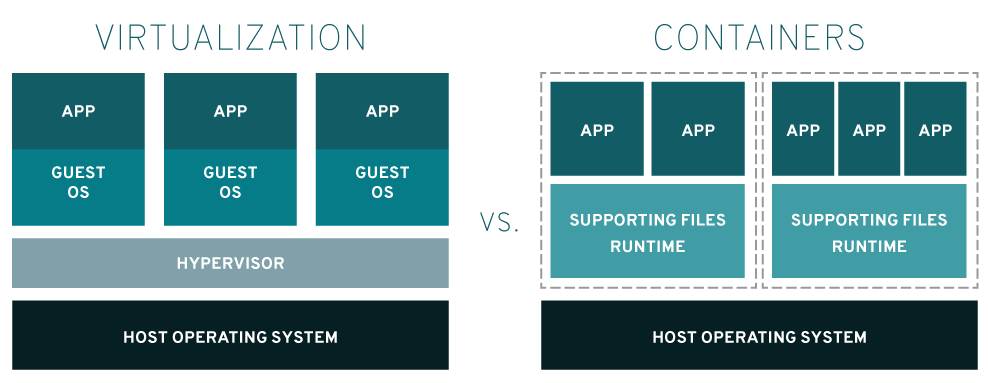
\includegraphics[width=1\textwidth]{kuvat/virtualization_vs_containers.png}
\caption{Täysi virtualisointi vs. käyttöjärjestelmätason virtualisointi~\cite{redhat:virtualization_vs_containers}}
\label{virtualization_vs_containers_image} 
\end{figure}

\section{Järjestelmän ja sovellusten konfiguraatio}\label{sovellusten_konfiguraatio}

\subsection{Autentikaatio}\label{autentikaatio}
Autentikaatioprosessia vahventamalla pyritään suojautumaan ensisijaisesti hyökkäykseltä \ref{bruteforce}. Perinteiset keinot suojautua, kuten tarpeeksi vahvan salasanan valitseminen ovat toki tärkeitä, mutta autentikaatioprosessia on myös mahdollista vahventaa järjestelmän konfiguraatioilla ja työkaluilla.

Käyttäjien salasanoille voidaan asettaa rajoitteita. Tällaiset rajoitteet voivat olla liian lyhyiden, liian yksinkertaisten tai luonnollisten kielten sanoista muodostuvien salasanojen estäminen. Kirjautumisyrityskerroille voidaan asettaa yläraja tai salasanoille voidaan asettaa vanhenemisaikoja. Nämä tekniikat heikentävät huomattavasti hyökkäyksen \ref{bruteforce} onnistumismahdollisuuksia. Linuxilla näitä tekniikoita voi ottaa käyttöön autentikaatiojärjestelmää konfiguroimalla tiedostosta \textit{/etc/login.defs} tai PAM:n avulla (\textbf{P}luggable \textbf{A}uthentication \textbf{M}odules).~\cite{kemp2009linux}

SSH on yleisin protokolla hallinnoida Linux-palvelimia etänä ja estämällä \textit{root}-käyttäjän kirjautumisen SSH:n ylitse pienentää huomattavasti hyökkäyspinta-alaa. Pääkäyttäjän \textit{root}-käyttäjätunnus on aina sama useimmissa UNIX-tyyppisissä järjestelmissä, joten hyökkääjän tarvitsee enää arvata vain salasana hyökkäyksen onnistumiseksi. Ennen \textit{root}-käyttäjän kirjautumisen estoa jokin toinen käyttäjä tulisi lisätä \textit{/etc/sudoers}-tiedostoon, jotta operointi pääkäyttäjäoikeuksilla onnistuisi silti SSH:n välityksellä.~\cite{sshd}~\cite{sudo}

\begin{algorithm}[tbh]
\begin{minted}{sh}
# Ensin lisätään "esimerkki"-käyttäjä /etc/sudoers:n
# ja annetaan tälle täydet oikeudet
echo 'esimerkki ALL=(ALL) ALL' >> /etc/sudoers
# Tämän jälkeen avataan SSH-palvelimen konfiguraatiotiedosto
vi /etc/ssh/sshd_config
# Muutetaan rivi:
PermitRootLogin Yes
# Riviksi:
PermitRootLogin No
# Tämän jälkeen SSH-palvelin tulisi käynnistää uudelleen
# esimerkiksi komennolla (riippuu jakelusta)
systemctl restart sshd
\end{minted}
\caption{Root-käyttäjän kirjautumisen estäminen\label{alg:disable_root_login}}
\end{algorithm}
\newpage{}

\subsection{Käyttöoikeudet}\label{access_rights}
Käyttöoikeuksien hallinnalla on tarkoitus hallita sitä kuka saa käyttää tai nähdä resursseja. Linux-palvelinten näkökulmasta on tietoturvan kannalta järkevää antaa esimerkiksi HTTP-palvelimelle oikeudet päästä käsiksi vain HTTP-palvelimelle relevantteihin tiedostoihin eikä koko järjestelmään. Tällöin esimerkiksi onnistuneen HTTP-palvelimeen kohdistuneen hyökkäyksen \ref{injection} seuraukset ovat pienemmät.

Perinteisesti UNIX-tyyppisissä käyttöjärjestelmissä resurssien käyttöoikeuksia hallinnoidaan tiedostojärjestelmätasolla niin, että jokaisella tiedostolla on omistajakäyttäjä sekä omistajaryhmä. Tämän lisäksi tiedostolle voidaan asettaa kirjoitus-, luku-, ja suoritusoikeudet kolmelle eri käyttäjäryhmälle erikseen: omistajakäyttäjälle, omistajaryhmälle sekä muille. Tiedoston omistajuus ilmoitetaan yleensä notaatiolla \textit{käyttäjä:ryhmä} ja käyttäjäryhmäkohtaiset oikeudet joko numeerisella kolmen numeron sarjana (esim. \textit{755}) josta jokainen numero on väliltä 0-7 tai symbolisella 10 merkin merkkijonolla, joka ensimmäistä merkkiä lukuun ottamatta koostuu merkeistä \textbf{r} (\textbf{r}ead, lukuoikeus), \textbf{w} (\textbf{w}rite, kirjoitusoikeus, \textbf{x} (e\textbf{x}ecution, suoritusoikeus) tai \textbf{-} (ei oikeutta). Esimerkin numeerinen oikeuksien esitys \textit{755} kääntyisi symboliseksi esitykseksi \textit{-rwxr-xr-x}. Symbolisen esityksen ensimmäinen merkki kertoo tiedoston tyypin eikä suoranaisesti liity käyttöoikeuksiin. Tiedoston omistajuuksia voi hallinta komennolla \textit{chown} ja käyttöoikeuksia komennolla \textit{chmod}.

Numeerisen esityksen ensimmäinen numero ja symbolisen esityksen kolme ensimmäistä merkkiä (tiedoston tyyppimerkin jälkeen) kertovat mitä oikeuksia tiedoston omistajakäyttäjällä on. Edellä mainitun esimerkin tapauksessa omistajalla on täydet oikeudet eli kirjoitus-, luku-, sekä suoritusoikeus. Numeerisen esityksen keskimmäinen numero ja symbolisen esityksen kolme seuraavaa merkkiä kertovat mitä oikeuksia omistajaryhmällä on. Esimerkin tapauksessa omistajaryhmällä on oikeudet lukea ja suorittaa tiedostoa. Viimeinen numero sekä viimeiset kolme merkkiä edustavat sitä millaisia oikeuksia kaikilla muilla käyttäjillä on. Esimerkin tapauksessa heilläkin on oikeudet lukea sekä suorittaa tiedostoa.

Useimmat tiedostojärjestelmät tukevat tämän lisäksi tiedostojen ominaisuuksia (eng. \textit{File Attributes}), joilla voidaan määritellä lisäasetuksia tiedostojen oikeuksille. Esimerkiksi tiedostoille voidaan määrittää, että niitä ei voi poistaa tai muunnella. Komennolla \textit{chattr} voidaan hallita tiedostojen ominaisuuksia.

Tiedostojen käyttöoikeuksista päättää tiedoston omistajakäyttäjä tai \textit{root}-käyttäjä. Perinteinen UNIX-tyyppinen käyttöoikeuksien hallinta on vuosikymmeniä sitten kehitetty järjestelmä ja se saattaa olla moderniin palvelinylläpitoon liian vanhanaikainen. Tämän vuoksi on kehitetty esimerkiksi laajennetut tiedostojen ominaisuudet (eng. \textit{Extended File Attributes}) tai kokonaan erilaisia lähestymistapoja käyttöoikeuksien hallintaan kuten SELinux.~\cite{kalsi2018practical}

\subsubsection{SELinux}\label{selinux}
SELinux (Security Enhanced Linux) on alun perin NSA:n kehittämä laajennus Linux-kerneliin, joka on ollut osa Linux-kerneliä vuodesta 2003. SELinux antaa työkalut hallita käyttöoikeuksia tarkemmin. Tärkein konseptillinen ero perinteiseen UNIX-tyyppiseen käyttöoikeuksien hallintaan on se, että SELinux arkkitehtuurillisesti pakollista käyttöoikeuksien hallintaa (eng. \textit{Mandatory Access Control, MAC}) kun taas perinteinen UNIX-tyyppinen käyttöoikeuksien hallinta valinnaista käyttöoikeuksien hallintaa (eng. \textit{Discretionary Access Control, DAC}). SELinux pyrkii erottamaan tietoturvan toteutuksen tietoturvaan liittyvistä päätöksistä.

Tuki SELinuxille on Linux-kernelissä ja useimpiin Linux-jakeluihin SELinuxin hallinnointityökalut ovat saatavilla. Useimmissa RPM-pohjaisissa jakeluissa kuten Red Hat Enterprice Linuxissa hallinnointityökalut tulevat vakiona.~\cite{selinux}

\section{Monitorointi}\label{monitorointi}
Monitoroinnin tarkoitus ei ole niinkään suojautua kyberhyökkäykseltä vaan ennemminkin keino havaita se. Kun hyökkäys havaitaan, se voidaan keskeyttää. Linux-jakelut ja sovellukset säilövät lokinsa yleensä hakemistoon \textit{/var/log/}. Epäilyttäviä HTTP-pyyntöjä kuten hyökkäyksessä \ref{injection} usein muodostuu voi yrittää etsiä HTTP-palvelimen lokista. Käynnissä olevan hyökkäyksen \ref{bruteforce} voi tunnistaa etsimällä epäilyttäviä kirjautumisyrityksiä Systemd:n lokista komennolla \textit{journalctl} tai tiedostoista \textit{/var/log/secure} tai \textit{/var/log/auth} riippuen jakelusta. 

Linux Audit Framework on yksi tärkeimmistä työkaluista tietoturvan monitorointiin Linuxilla. Audit Frameworkin käyttäjätilan työkalulla \textit{aureport} voidaan laatia raportti tietoturvapoikkeamista. Mikäli SELinux on käytössä se tallentaa lokia tietoturvapoikkeamista omiin lokitiedostoihinsa.~\cite{xplg}

Koodilistauksessa~\ref{alg:secure} tunnistan epäilyttävän kirjautumisyrityksen parsimalla Systemd:n lokia, jonka jälkeen käytän palomuuria sulkeakseni liikenteen kyseisestä lähteestä keskeyttääkseni hyökkäysyrityksen.

\begin{algorithm}[tbh]
\begin{minted}{sh}
# Parsitaan Systemd:n lokia
journalctl -xe | grep -i "failed password"
# Komento tulostaa seuraavat rivit
marras 19 04:56:40 r5 sshd[2256116]: Failed password for invalid user
epailyttava from 192.168.8.124 port 19204 ssh2
marras 19 04:56:44 r5 sshd[2256116]: Failed password for invalid user
epailyttava from 192.168.8.124 port 19204 ssh2
marras 19 04:56:47 r5 sshd[2256116]: Failed password for invalid user
epailyttava from 192.168.8.124 port 19204 ssh2
# Estetään liikenne kyseisestä lähteestä palomuurilla
ufw deny from "192.168.8.124"
\end{minted}
\caption{Epäilyttävän kirjautumisyrityksen tunnistus.\label{alg:secure}}
\end{algorithm}
